\renewcommand{\thefootnote}{\fnsymbol{footnote}}

\chapter[First theorem of welfare economics]%
 {First theorem of welfare economics}%
\label{ch:L9}

% 3) Reset things so later footnotes go back to 1, 2, 3, …
%\setcounter{footnote}{0}
\renewcommand{\thefootnote}{\arabic{footnote}}

\section{A preliminary lemma}\label{sec:L8-intro}

We start with a preliminary lemma. All the proofs here are by contradiction. The logic of these proofs is as follows. We want to prove some statement \( S \). We assume that \( S \) is false, and we show that this assumption leads to a contradiction, that is, some conclusion of the type \( C \) and \textbf{not} \( C \), which is impossible. Therefore, \( S \) must be true.

\begin{lemma}\label{lem:lns}
    Assume preferences \( \succsim_i \) are locally non-satiated. Let \( x_i \in D_i (p,e_i) \). If \( x'_i \succsim_i x_i \), then \( p \cdot x'_i \ge p \cdot x_i \).
\end{lemma}

\begin{proof}
    Suppose not. Then \( p \cdot x'_i < p \cdot x_i \). By local non-satiation, there exists \( x''_i \) such that \( \|x''_i - x'_i\| < \varepsilon \) and \( x''_i \succ_i x'_i \). By choosing \( \varepsilon \) small enough, we can ensure that \( p \cdot x''_i < p \cdot x_i \). But then \( x''_i \in B(e_i,p) \) and \( x''_i \succ_i x_i \), by transitivity, contradicting the fact that \( x_i \in D_i (e_i, p) \).
\end{proof}

\subsection{The main result}

\begin{theorem}\label{thm:fftwe} (\textbf{First fundamental theorem of welfare economics}) If preferences in the economy \( E \) are locally non-satiated, then every allocation selected by a Walrasian equilibrium with transfers is Pareto optimal. That is,

    \[
        x \in R^{WT} (E) \quad \Longrightarrow \quad x \quad \text{is Pareto optimal}.
    \]
\end{theorem}

\begin{proof}
    Let \(E\) be an economy and suppose that \(x \in R^{WT}(E)\).
    Then there exist strictly positive prices \(p\) and transfers
    \((T_i)_{i\in I}\) such that, for every individual \(i\),
    \[
        x_i \in D_i(e_i + T_i,p),
    \]
    that is, \(x_i\) is a most preferred bundle in the budget set
    \(B(e_i+T_i,p)\).

    Suppose, towards a contradiction, that \(x\) is not Pareto optimal.
    Then there exists a feasible allocation \(x'\) such that
    \(x'_i \succsim_i x_i\) for all \(i\), and
    \(x'_j \succ_j x_j\) for some individual \(j\).
    By the Lemma \ref{lem:lns}, local non-satiation implies
    \[
        p\cdot x'_i \ge p\cdot x_i \quad \forall i,
        \qquad
        p\cdot x'_j > p\cdot x_j.
    \]
    Summing over all individuals,
    \[
        \sum_{i\in I} p\cdot x'_i > \sum_{i\in I} p\cdot x_i.
    \]

    On the other hand, feasibility of \(x'\) implies
    \[
        \sum_{i\in I} x'_i \le \sum_{i\in I} e_i
        = \sum_{i\in I} x_i,
    \]
    since \(x\) is feasible as well.
    Multiplying the inequality
    \(\sum_i (x'_i - x_i) \le 0\)
    by the strictly positive price vector \(p\) yields
    \[
        \sum_{i\in I} p\cdot x'_i
        \le \sum_{i\in I} p\cdot x_i,
    \]
    contradicting the strict inequality obtained above.
    Hence no such \(x'\) exists, and
    \(x\) is Pareto optimal.
\end{proof}

Let us discuss why Local non-satiation is necessary for Theorem \ref{thm:fftwe} to hold. Individual \( 1 \) has \textquote{thick} indifference curves, thus violating local non-satiation. The allocation \( x \) is not Pareto optimal, since we can find another feasible allocation \( x' \) that makes individual \( 2 \) strictly better off without making individual \( 1 \) worse off. However, \( x \) can still be supported as a Walrasian equilibrium with transfers at prices \( p \). Thus, without local non-satiation, Theorem \ref{thm:fftwe} fails.

\begin{figure}[H]
    \begin{center}
        \tikzset{every picture/.style={line width=0.75pt}} %set default line width to 0.75pt        

        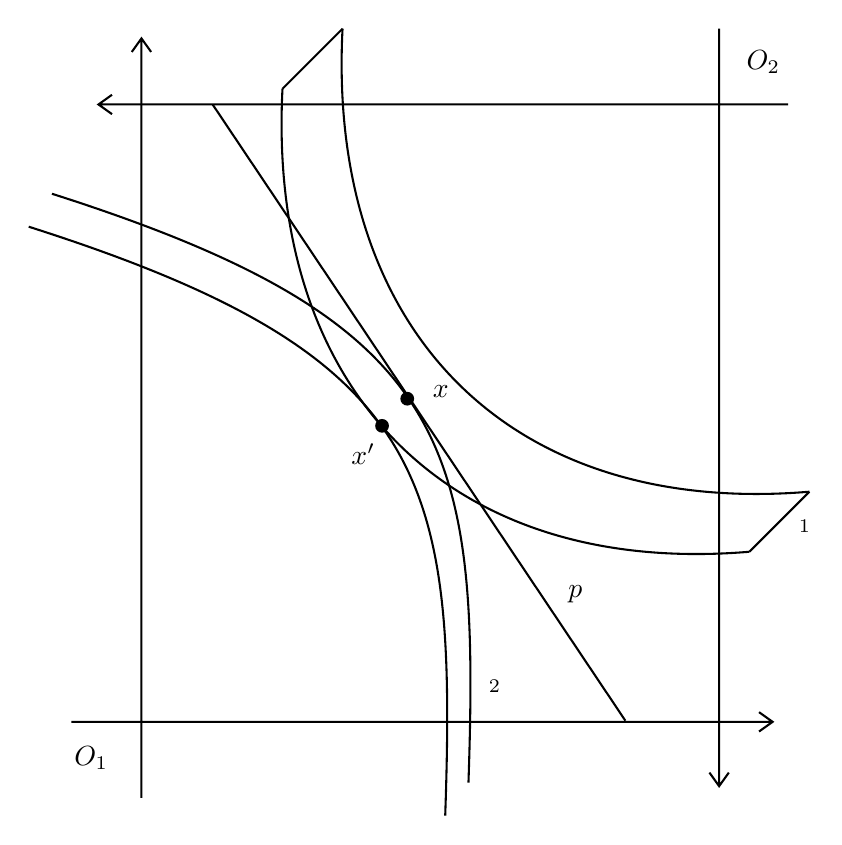
\begin{tikzpicture}[x=0.70pt,y=0.70pt,yscale=-1,xscale=1]
            %uncomment if require: \path (0,443); %set diagram left start at 0, and has height of 443

            %Shape: Axis 2D [id:dp22115699468612893] 
            \draw  (140,370.4) -- (502,370.4)(176.2,17.6) -- (176.2,409.6) (495,365.4) -- (502,370.4) -- (495,375.4) (171.2,24.6) -- (176.2,17.6) -- (181.2,24.6)  ;
            %Shape: Axis 2D [id:dp32207533916759135] 
            \draw  (510,51.7) -- (154,51.7)(474.4,403.6) -- (474.4,12.6) (161,56.7) -- (154,51.7) -- (161,46.7) (479.4,396.6) -- (474.4,403.6) -- (469.4,396.6)  ;
            %Curve Lines [id:da8559403196511832] 
            \draw    (249,43.6) .. controls (241,199.6) and (335,295.6) .. (490,282.6) ;
            %Curve Lines [id:da37662840950707166] 
            \draw    (280,12.6) .. controls (272,168.6) and (366,264.6) .. (521,251.6) ;
            %Straight Lines [id:da5642668535456735] 
            \draw    (249,43.6) -- (280,12.6) ;
            %Straight Lines [id:da9097139754709688] 
            \draw    (490,282.6) -- (521,251.6) ;
            %Curve Lines [id:da09819389723996741] 
            \draw    (130,97.8) .. controls (337,163.8) and (351,225.8) .. (345,401.8) ;
            %Shape: Circle [id:dp16582666368555876] 
            \draw  [fill={rgb, 255:red, 0; green, 0; blue, 0 }  ,fill opacity=1 ] (310.4,203.6) .. controls (310.4,201.94) and (311.74,200.6) .. (313.4,200.6) .. controls (315.06,200.6) and (316.4,201.94) .. (316.4,203.6) .. controls (316.4,205.26) and (315.06,206.6) .. (313.4,206.6) .. controls (311.74,206.6) and (310.4,205.26) .. (310.4,203.6) -- cycle ;
            %Shape: Circle [id:dp20605667579120546] 
            \draw  [fill={rgb, 255:red, 0; green, 0; blue, 0 }  ,fill opacity=1 ] (297.4,217.6) .. controls (297.4,215.94) and (298.74,214.6) .. (300.4,214.6) .. controls (302.06,214.6) and (303.4,215.94) .. (303.4,217.6) .. controls (303.4,219.26) and (302.06,220.6) .. (300.4,220.6) .. controls (298.74,220.6) and (297.4,219.26) .. (297.4,217.6) -- cycle ;
            %Curve Lines [id:da6954752398238686] 
            \draw    (118,114.8) .. controls (325,180.8) and (339,242.8) .. (333,418.8) ;
            %Straight Lines [id:da49767621503014337] 
            \draw    (213,51.8) -- (426,369.8) ;

            % Text Node
            \draw (140,381.4) node [anchor=north west][inner sep=0.75pt]    {$O_{1}$};
            % Text Node
            \draw (487,22.4) node [anchor=north west][inner sep=0.75pt]    {$O_{2}$};
            % Text Node
            \draw (514,264.4) node [anchor=north west][inner sep=0.75pt]    {$\succsim _{1}$};
            % Text Node
            \draw (325,195.4) node [anchor=north west][inner sep=0.75pt]    {$x$};
            % Text Node
            \draw (283,225.4) node [anchor=north west][inner sep=0.75pt]    {$x'$};
            % Text Node
            \draw (354,347.4) node [anchor=north west][inner sep=0.75pt]    {$\succsim _{2}$};
            % Text Node
            \draw (395,298.4) node [anchor=north west][inner sep=0.75pt]    {$p$};
        \end{tikzpicture}
        \label{fig:lns-fwelf}
        \caption{Local Non-Satiation is necessary for the First Welfare Theorem.}
    \end{center}
\end{figure}

There are two ways to interpret Theorem \ref{thm:fftwe}. A \textit{logical} one, and a \textit{positive} one. The logical interpretation is the following. One might want to answer

First, it shows that the Walrasian equilibrium with transfers is an \textit{efficient} allocation rule, in the sense that it always selects Pareto optimal allocations. Second, it shows that if we observe an allocation that is not Pareto optimal, then we can conclude that this allocation could not have arisen as a Walrasian equilibrium with transfers.

\paragraph{Things to read.} This lecture is based on \citet[pp. 545-550]{mas-colellMicroeconomicTheory1995}.

\section{Exercises}

hey.

\bibliographystyle{apacite}  % or another  style
\bibliography{references} % .bib file goes in ./bib/